\noindent
\label{sec:dataanalytics}
%Machine learning techniques are becoming increasingly important for many data-analytics models, and healthcare data analysis is no exception. 
\noindent
Machine learning methods such as deep neural networks have delivered remarkable results in data-analytics for a wide range of application domains, including healthcare. However, their training requires large data-sets which might be containing sensitive information that need to be be protected from \emph{model inversion} attack~\cite{Fredrikson:2015:MIA:2810103.2813677} and adversaries with access to model parameters and knowledge of the training procedure. This problem is addressed within the framework of differential privacy~\cite{Abadi:2016:DLD:2976749.2978318,Phan:2016:DPP:3015812.3016005}. Machine learning algorithms typically operate on data in the form of a matrix where e.g. rows correspond to features and columns correspond to samples. The particular problem in the context of matrix-valued data is to protect a machine learning algorithm, under differential privacy framework, from an adversary who seeks to gain an information about the data from an algorithm's output by perturbing the value in an element of the training data matrix. Despite the fact that random noise adding mechanism has been widely studied in privacy-preserving machine learning, there remains the challenge of studying privacy-utility trade-off for matrix-valued query functions. Our recent work~\cite{Kumar/IWCFS2019} has suggested a novel entropy based approach for resolving the privacy-utility trade-off for real-valued data matrices. The study in~\cite{Kumar/IWCFS2019}  mathematically derives the probability density function of noise that minimizes the expected noise magnitude together with satisfying sufficient conditions for $(\epsilon,\delta)-$differential privacy.

\subsubsection{An Optimal $(\epsilon,\delta)-$Differentially Private Noise for Real-Valued Matrices}
Consider a data-set consisting of $N$ number of samples with each sample having $p$ number of attributes represented by a matrix $\mathrm{Y} \in \mathbb{R}^{p \times N}$. A given machine learning algorithm, training a model using data matrix $\mathrm{Y}$, can be represented by a mapping, $\mathcal{A}: \mathbb{R}^{p \times N} \rightarrow \mathbf{M}$, where $\mathbf{M}$ is the model space.  
\begin{definition}[A Private Algorithm]\label{definition_private_algorithm}
Let $\mathcal{A}^+ : \mathbb{R}^{p \times N} \rightarrow Range(\mathcal{A}^+)$ be a mapping defined as
\begin{IEEEeqnarray}{rCl}
\mathcal{A}^+\left(\mathrm{Y}\right) & = & \mathcal{A}\left(\mathrm{Y} + \mathrm{V}\right),\;  \mathrm{V} \in \mathbb{R}^{p \times N}
\end{IEEEeqnarray}  
where $\mathrm{V}$ is a random noise matrix with $f_{\mathrm{v}_j^i}(v)$ being the probability density function of its $(j,i)-$th element $\mathrm{v}_j^i$; $\mathrm{v}_j^i$ and $\mathrm{v}_j^{i^{\prime}}$ are independent from each other for $i \neq i^{\prime}$; and $\mathcal{A}(\cdot)$ is a given mapping representing a machine learning algorithm. 
\end{definition}  
\begin{definition}[$d-$Adjacency for Data Matrices]\label{def_adjacency_matrices}
Two matrices $\mathrm{Y},\mathrm{Y}^{\prime} \in \mathbb{R}^{p \times N}$ are $d-$adjacent if for a given $d  \in \mathbb{R}_{+}$, there exist $i_0 \in \{1,2,\cdots,N\}$ and $j_0 \in \{1,2,\cdots,p\}$ such that $\forall i \in \{1,2,\cdots,N\}, j \in \{1,2,\cdots,p\}$,
 \begin{IEEEeqnarray*}{rCl}
\left | \mathrm{y}^i_j - \mathrm{y}^{\prime i}_j \right | & \leq & \left\{ \begin{array}{cc}
d, & \mbox{if $i = i_0,j = j_0$} \\
0, & \mbox{otherwise}
  \end{array} \right.
\end{IEEEeqnarray*}    
where $\mathrm{y}^i_j$ and $\mathrm{y}^{\prime i}_j$ denote the $(j,i)-$th element of $\mathrm{Y}$ and $\mathrm{Y}^{\prime}$ respectively. Thus, $\mathrm{Y}$ and $\mathrm{Y}^{\prime}$ differ by only one element and the magnitude of the difference is upper bounded by $d$. 
\end{definition} 
\begin{definition}[$(\epsilon,\delta)-$Differential Privacy for $\mathcal{A}^+$]\label{def_differential_privacy}
The algorithm $\mathcal{A}^+\left(\mathrm{Y}\right)$ is $(\epsilon,\delta)-$differentially private if
 \begin{IEEEeqnarray}{rCl}
\label{eq_differential_privacy}  Pr\{ \mathcal{A}^+\left(\mathrm{Y}\right) \in \mathcal{O} \} & \leq & \exp(\epsilon) Pr\{ \mathcal{A}^+\left(\mathrm{Y}^{\prime}\right)) \in \mathcal{O} \} + \delta \IEEEeqnarraynumspace
\end{IEEEeqnarray}     
for any measurable set $\mathcal{O} \subseteq  Range(\mathcal{A}^+) $ and for $d-$adjacent matrices pair $(\mathrm{Y},\mathrm{Y}^{\prime})$. Here, $Pr\{ \cdot \}$ is the probability taken over the randomness used by algorithm.
\end{definition} 
\begin{result}[An Optimal $(\epsilon,\delta)-$Differentially Private Noise]\label{result_optimal_noise_epsilon_delta_privacy}
The probability density function of noise that minimise the expected noise magnitude together with satisfying the sufficient conditions for $(\epsilon,\delta)-$differential privacy of $\mathcal{A}^+$ is given as
\begin{IEEEeqnarray}{rCl}
\label{eq_optimal_density_epsilon_delta_privacy} f_{\mathrm{v}_j^i}^*(v) &  = & \left \{\begin{array}{cl}  \delta Dirac\delta(v), & v = 0 \\
 (1- \delta)\frac{\displaystyle \epsilon}{\displaystyle  2 d} \exp(-\frac{\displaystyle  \epsilon}{\displaystyle   d} |v|), & v \in   \mathbb{R} \setminus \{0\}
\end{array} \right.
\end{IEEEeqnarray}  
where $Dirac\delta(v)$ is Dirac delta function satisfying $\int_{-\infty}^{\infty}Dirac\delta(v)\: \dd v = 1$. The optimal value of expected noise magnitude is given as
\begin{IEEEeqnarray}{rCl}
\label{eq_optimal_noise_magnitude_epsilon_delta_privacy} E_{f_{\mathrm{v}_j^i}^*}\left[|v|\right] & = & (1-\delta) \frac{d}{\epsilon}.
\end{IEEEeqnarray}  
\end{result}
\begin{IEEEproof}
The proof follows from~\cite{Kumar/IWCFS2019}.
 \end{IEEEproof}


\subsubsection{Differentially Private Distributed Deep Learning}
The post-processing invariant property~\cite{DBLP:journals/fttcs/DworkR14} of differential privacy allows one to compose a global private deep model from local private deep models.

%\begin{figure}[!h]
%\centering
% \scalebox{1}{
%\begin{tikzpicture}[multilayer = 3d]
%\SetLayerDistance{2}
%\Plane[x=0,y=0,width=4,height=2,RGB,color={235,235,235},InBG=True,N%oBorder=True,layer=1]
%\Vertex[size=1,x=1,y=1,label=$\mathrm{Y}^1$,fontscale=1,layer=1]{y}
%\Vertex[size=1,x=3,y=1,label=$\mathrm{Y}^2$,fontscale=1,layer=1,col%or=orange!50!white]{y2}
%\Plane[x=0,y=0,width=4,height=2,RGB,color={255,184,184},InBG=True,NoBorder=True,layer=2]
%\Vertex[size=1.5,x=1,y=1,label=$\mathrm{Y}^{1}+\mathrm{V}^{1}$,fontscale=1,layer=2]{y+}
%\Vertex[size=1.5,x=3,y=1,label=$\mathrm{Y}^{2}+\mathrm{V}^{2}$,fontscale=1,layer=2,color=orange!50!white]{y2+}
%\Edge[color=blue,lw=1,bend=0](y+)(y)
%\Edge[color=blue,lw=1,bend=0,color=orange](y2+)(y2)
%\Plane[x=0,y=0,width=4,height=2,RGB,color={235,235,235},InBG=True,NoBorder=True,layer=3]
%\Vertex[size=1.5,x=1,y=1,label=$\mathcal{A}^+\left(\mathrm{Y}^1\right)$,fontscale=1,layer=3,color=red!30!white]{M}
%\Vertex[size=1.5,x=3,y=1,label=$\mathcal{A}^+\left(\mathrm{Y}^2\right)$,fontscale=1,layer=3,color=red!30!white]{M2}
%\Edge[color=red,lw=1,bend=0](y+)(M)
%\Edge[color=red,lw=1,bend=0](y2+)(M2)
%\Plane[x=0,y=0,width=4,height=2,RGB,color={235,235,235},InBG=True,NoBorder=True,layer=4]
%\Vertex[size=1.75,x=2,y=1,label=global model,fontscale=1,layer=4,color=red!30!white]{fuzzy_rules}
%\Edge[color=blue,lw=1,bend=0,color=red](M)(fuzzy_rules)
%\Edge[color=blue,lw=1,bend=0,color=red](M2)(fuzzy_rules)
%\Text[x=3.75,y=1.8,style={draw,rectangle},fontsize=\small,layer=1]{1.}
%\Text[x=5.1,y=1.8,style={color=blue},width=2cm,fontsize=\small,layer=1]{local data}
%\Text[x=3.75,y=1.8,style={draw,rectangle},fontsize=\small,layer=2]{2.}
%\Text[x=6.1,y=1.60,style={color=blue},width=4cm,fontsize=\small,layer=2]{privacy wall $(\epsilon,\delta)-$differential privacy}
%\Text[x=3.75,y=1.8,style={draw,rectangle},fontsize=\small,layer=3]{3.}
%\Text[x=5.35,y=1.6,style={color=blue},width=2.5cm,fontsize=\small,layer=3]{local private deep models}
%\Text[x=3.75,y=1.8,style={draw,rectangle},fontsize=\small,layer=4]{4.}
%\Text[x=5.35,y=1.6,style={color=blue},width=2.5cm,fontsize=\small,layer=4]{global private deep model}
%\end{tikzpicture}
%}

\begin{figure}[h!]
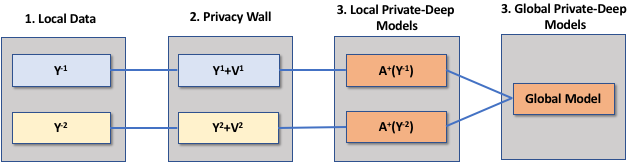
\includegraphics[width=\columnwidth]{images/privacypreserving.png}
\caption{A structural representation of the differentially private distributed learning for deep models.}
\label{fig_structural_representation_distributed_differential_private}
\end{figure}

%\caption{A structural representation of the differentially private distributed learning for deep models.}
%\label{fig_structural_representation_distributed_differential_private}
%\end{figure} 
The distributed form of differentially private deep learning is represented in Fig.~\ref{fig_structural_representation_distributed_differential_private} where a privacy wall is inserted between training data and the globally shared data. The privacy wall uses noise adding mechanisms to attain differential privacy for each participant's private training data. Therefore, the adversaries have no direct access to the training data. 
     



